\chapter{Confirmation du rôle de l'interférence: modification de la structure
des populations et observation de l'accès aux ressources}
\chaptermark{Confirmation du rôle de l'interférence}
\label{chap:sm}

\vspace{5cm}

\section{Introduction}

\lettrine[lines=3]{N}{otre} étude de l'effet des interactions entre individus
dans la dynamique des populations structurées nous a mené dans le Chapitre
\ref{chap:sp} à proposer la
compétition par interférence comme mécanisme responsable de la structuration
multimodale de nos populations expérimentales de collemboles \textit{Folsomia
candida} (voir aussi Annexe \ref{Ann:SP}). Au cours du Chapitre
\ref{chap:amnat} (voir aussi Annexe \ref{An:AmNat}), nous avons étudié dans un
modèle théorique les conséquences d'une compétition par interférence plus ou moins intense sur la dynamique d'une population structurée où la compétition par
exploitation entre également en jeu. Nous avons montré qu'une compétition par
interférence suffisamment intense pouvait être à l'origine d'une stabilisation
des cycles de génération dominés par les juvéniles, puis de l'apparition de
cycles de plus longue période au cours des quels des individus parviennent à
atteindre de très grandes tailles, et où la population a une structure
multimodale. Ces deux études semblent donc montrer que la compétition par
interférence est un mécanisme suffisant pour l'apparition de distributions
multimodales dans des populations structurées par la taille, et la survie
d'individus à des tailles bien supérieures à leur taille à maturité.

Suite aux résultats de notre étude théorique, nous avons voulu vérifier dans nos
populations expérimentales quel était le rôle précis des individus de
différentes tailles dans les dynamiques des structures observées, afin de
pouvoir affirmer le rôle de la compétition par interférence avec plus de certitudes.
Pour ce faire, nous avons mené deux expériences en parallèle. Dans une première
expérience nous sommes intervenus sur des populations dont la dynamique semblait
stable en perturbant la structure de la population afin d'en observer le retour
à l'équilibre et de pouvoir comparer la situation finale à celle avant la
perturbation. Cette expérience a été réalisée sur les deux clones étudiés
jusque-là, HA et TO.

Dans une seconde expérience nous nous sommes intéressés aux comportements
d'accès à la ressource dans les populations. Nous avons réalisé une série
d'observations en temps réel dans les populations afin de mieux comprendre
comment la ressource était partagée entre les individus d'une population. Ces
observations ont été réalisées dans certaines des populations de la première
expérience. Elles ont permis de comparer la distribution en taille des individus
accédant à la ressource à celle de l'ensemble de la population au moment de
l'observation. Cette comparaison a mis en évidence un accès différentiel en
fonction de la taille avec un biais quasi-systématique en faveur des individus
les plus grands dans l'accès à la ressource. 

\section{Matériel et méthodes}

\subsection{Perturbation de la structure d'une population}

Dans la première expérience, nous avons suivis des populations de collemboles
\textit{Folsomia candida} jusqu'à stabilisation de leur structure, puis nous
avons perturbé la structure afin d'observer le retour à un régime permanent. 

\subsubsection{Les populations étudiées}

Nous avons élevé et dénombré régulièrement $16$ populations de collemboles, $8$
du clone HA et $8$ du clone TO, pendant un an jusqu'à stabilisation de la
structure. Les populations ont été élevées à $21\degres$C dans les conditions
décrites dans le Chapitre \ref{chap:method}. Les populations ont été mesurées
régulièrement pour suivre leur structure en suivant également la méthode de
phénotypage haut débit présentée précédemment (voir Chapitre \ref{chap:method}
Section \ref{sec:bpsensor} et Annexe \ref{Ann:bpsensor}).

\subsubsection{Perturbation de la structure}

\paragraph{Témoins} Après 12 mois, nous considérons que la période transitoire
de la dynamique est terminée. La perturbation de la structure que nous imposons
aux populations fait intervenir un changement de boite d'élevage. Afin de
vérifier l'impact d'un changement de boite sur la dynamique de la structure
d'une population, nous conservons deux témoins pour chacun des clones pour les
quels la structure n'est pas modifiée mais la population est intégralement
transférée dans une nouvelle boite d'élevage.

\paragraph{Clone HA} Avant la perturbation de la structure les populations du
clone HA ont toutes convergé vers une distribution tri-modale de la taille
corporelle. Nous avons donc réalisé trois traitements différents, chacun sur
deux populations. Chaque traitement consiste à diviser une population en deux en
fonction de la taille des individus. La structure de la population étant séparée
en trois modes, un des modes est prélevé et isolé dans une nouvelle boite
d'élevage, tandis que les deux autres sont conservés ensemble et également
transférés dans une nouvelle boite.

Les trois modes des distributions sont désignés respectivement par les lettres J
(ou Je) pour les juvéniles, M (ou Mo) pour le premier mode d'adultes de
taille moyenne, et G (ou Gd) pour le mode d'adultes de grande taille. Les
différents traitements consistent donc à \begin{enumerate*}[label=(\roman*), before=\unskip{ : }, itemjoin={{ ; }},
itemjoin*={{ ; et }}]
\item isoler la cohorte Je et conserver les cohortes M et G dans une population
MG
\item isoler la cohorte Mo et conserver les cohortes J et G dans une population
JG
\item isoler la cohorte Gd et conserver les cohortes J et M dans une population
JM (Figure \ref{fig:SM0}).
\end{enumerate*} 
Après la séparation des cohortes, les populations nouvellement fondées sont
replacées dans les conditions d'élevage habituelles et dénombrées et mesurées
régulièrement pendant $15$ mois pour observer la période de transition et le
retour à une structure stable. 

\begin{figure}[!ht]
\begin{center}
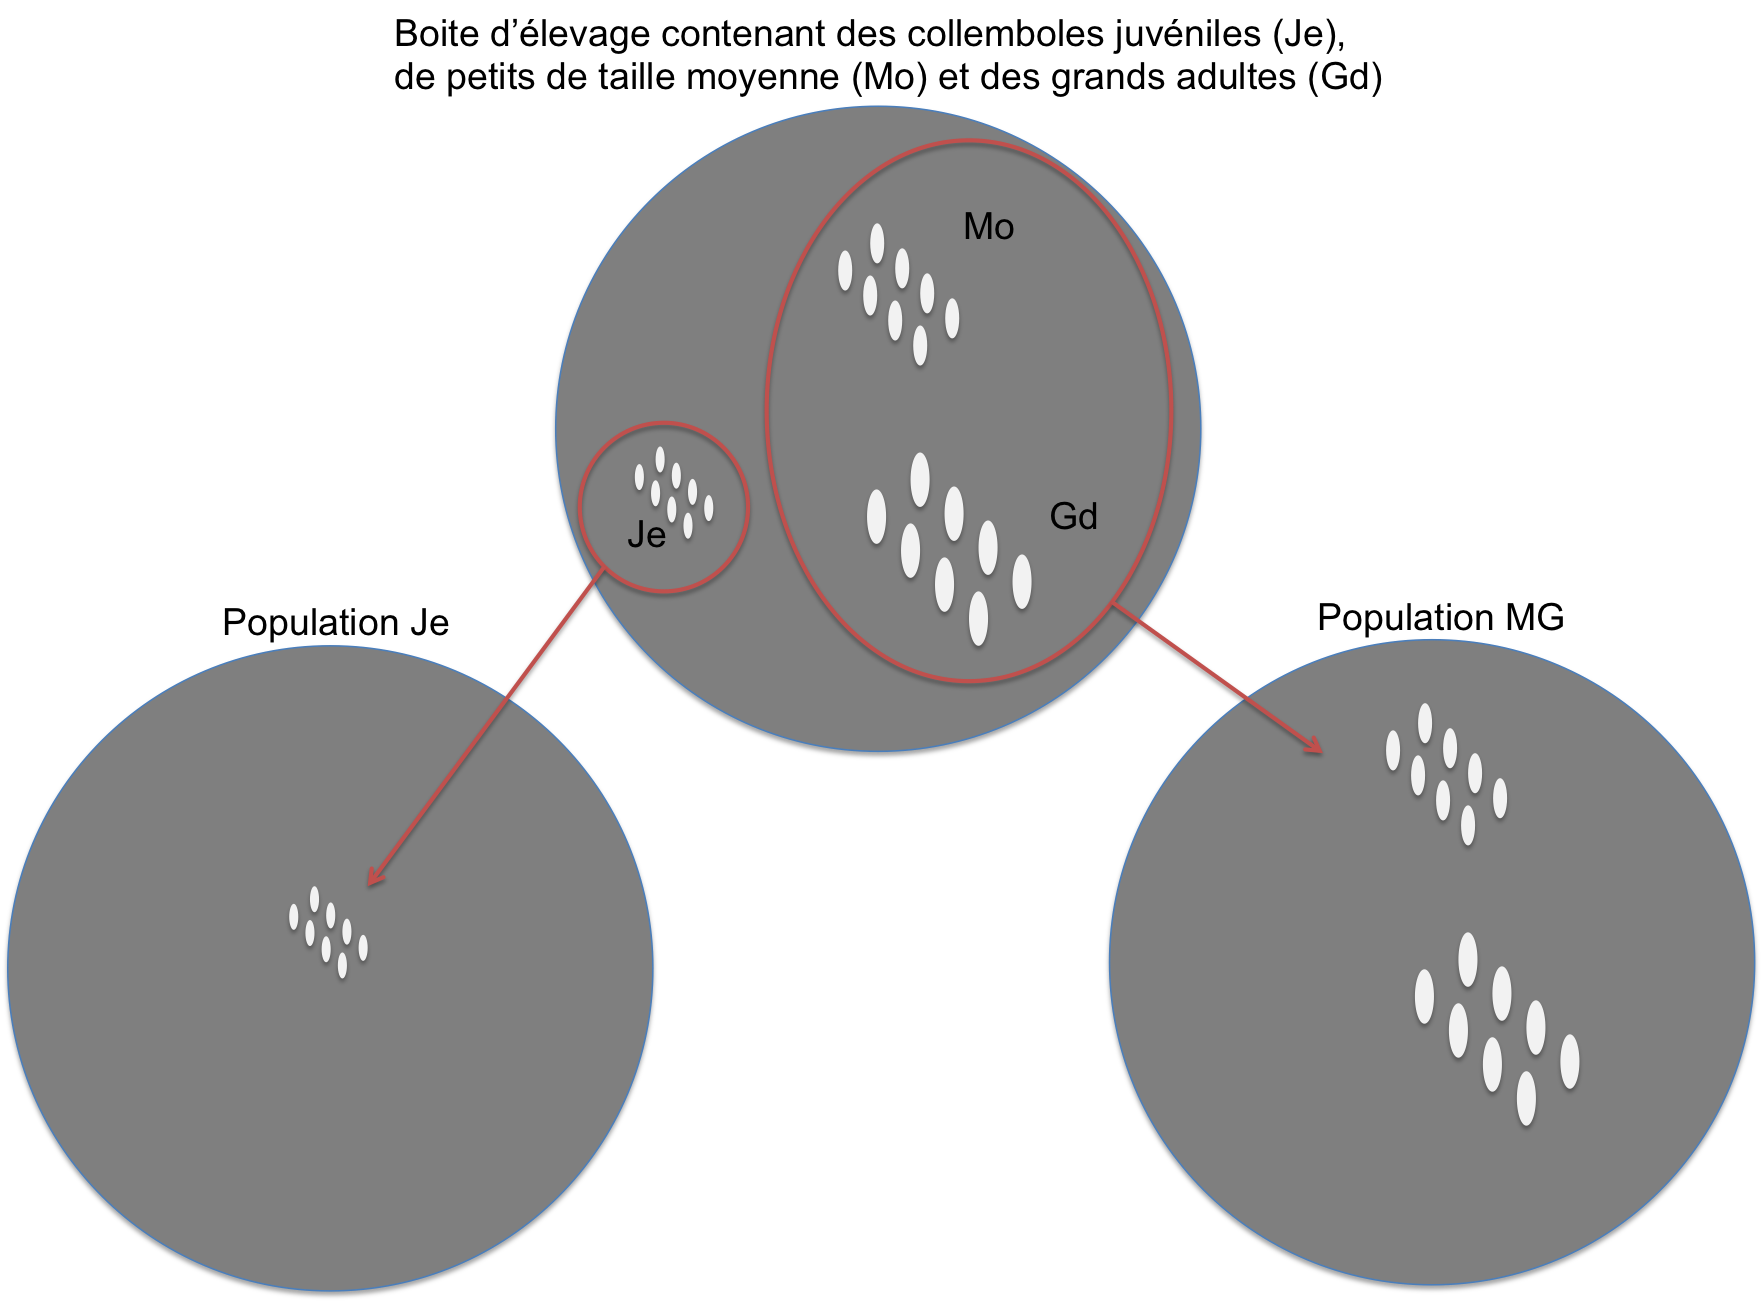
\includegraphics[width=1\textwidth]{1_CorpsDeThese/Resumes/Fig/SM00}
\caption[\lofimage{1_CorpsDeThese/Resumes/Fig/SM01}Exemple de
séparation d'une population]{Exemple de
séparation d'une population pour un traitement Je - MG.}
\label{fig:SM0}
\end{center}
\end{figure}


\paragraph{Clone TO} Contrairement au clone HA, les populations du clone TO ont
convergé au cours de la première phase de l'expérience vers des structures
bimodales. L'analyse des populations HA a montré que les adultes se répartissent
en moyenne en $\frac{2}{3}$ de petits adultes et $\frac{1}{3}$ de grands
adultes. Afin de conserver des manipulations comparables entre les clones HA et
TO, et mettre les nouvelles populations dans des conditions similaires entre les
deux clones, nous avons décidé de séparer la cohorte d'adultes en un groupe
contenant deux tiers des individus (M) et un groupe contenant le tiers restant
(G) afin de suivre les mêmes traitements que pour le clone HA. Les individus
sont choisis au hasard pour être attribué à M ou G.
Ainsi, les traitements sont \begin{enumerate*}[label=(\roman*), before=\unskip{ : }, itemjoin={{ ; }},
itemjoin*={{ ; et }}]
\item isoler la cohorte Je et conserver ensemble tous les adultes (MG)
\item isoler deux tiers des adultes (Mo) et conserver les cohortes J et le reste
des adultes G (JG)
\item isoler un tiers des adultes (Gd) et conserver les cohortes J et deux tiers
des adultes M (JM).
\end{enumerate*} 
Les nouvelles populations sont suivies pendant $15$ mois pour observer la phase
transitoire et observer le nouvel équilibre. 

\begin{figure}[!ht]
\begin{center}
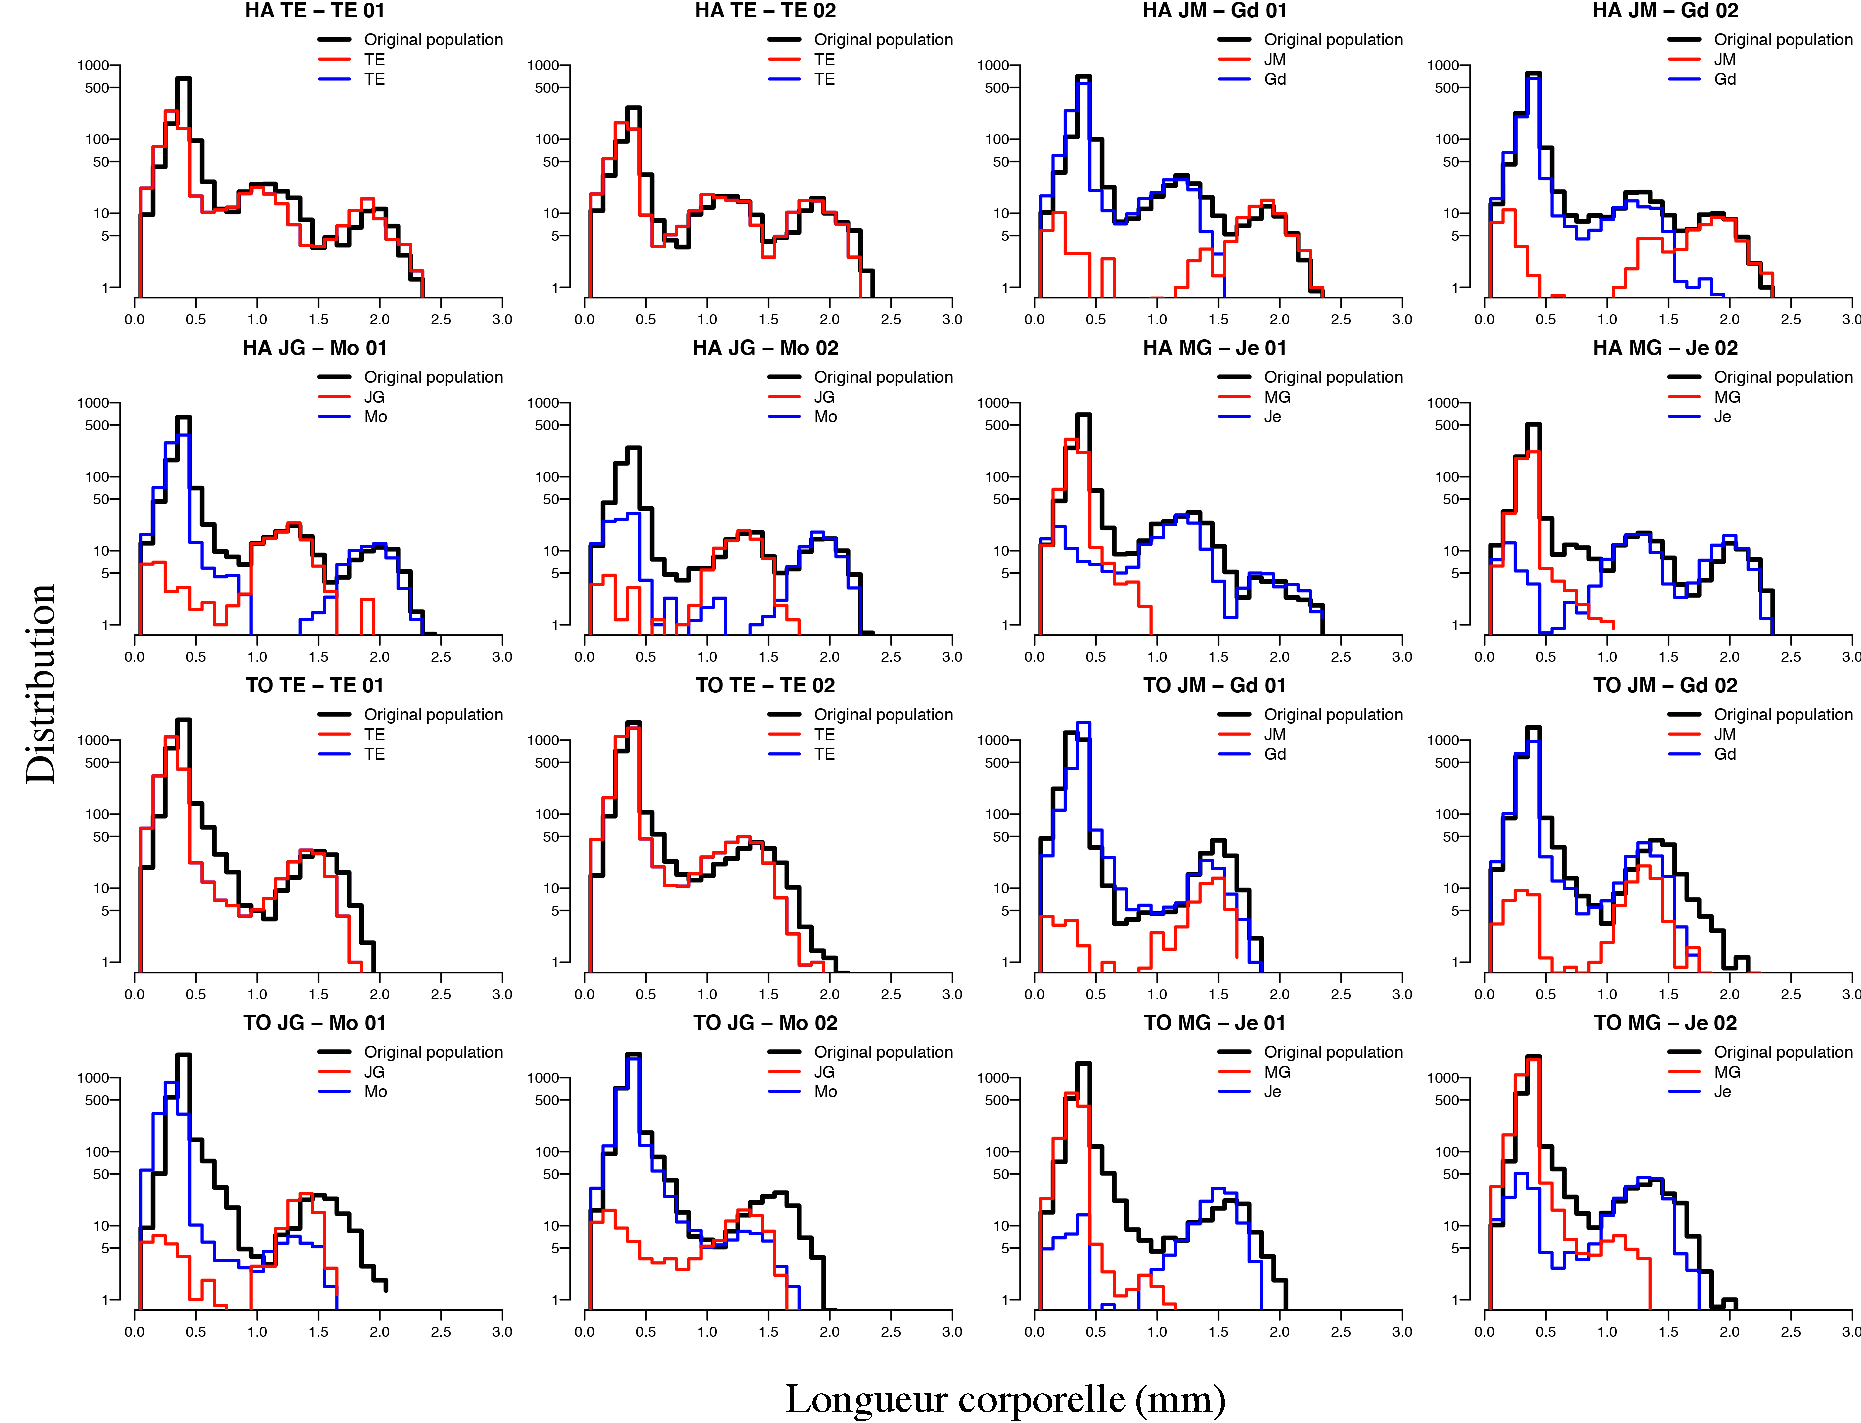
\includegraphics[width=1\textwidth]{1_CorpsDeThese/Resumes/Fig/SM01}
\caption[\lofimage{1_CorpsDeThese/Resumes/Fig/SM01}Séparation des
populations]{Résultat de la séparation des populations en deux en fonction de
la taille des individus. La ligne noire est la population d'origine, les lignes
bleues et rouges sont les populations séparées. Je, Mo et Gd se réfèrent
respectivement aux cohortes J, M et G.}
\label{fig:SM1}
\end{center}
\end{figure}

Afin de vérifier le résultat des séparations des populations en deux, nous avons
tracé pour chaque population, sur un même graphique, la distribution de la
taille dans la population d'origine et dans chacune des deux nouvelles
populations. L'ensemble des graphiques obtenus est présenté sur la Figure
\ref{fig:SM1}

\subsubsection{Analyse des dynamiques}

Les dynamiques des structures avant et après perturbation sont analysées grâce
aux diagrammes structure-temps (Chapitre \ref{chap:method} Section \ref{sec:stdiag} et
Annexe \ref{Chap:STDiag}).
Les structures après stabilisation sont alors comparées aux structures avant perturbation et
aux autres traitements. 

\subsection{Accès à la ressource}

Dans la seconde expérience de cette étude, nous réalisons une série d'analyses
\textit{in-situ} des comportements d'accès aux ressources.

\subsubsection{Observations comportementales}

La ressource est composée d'une pastille de quelques millimètres de diamètre de
levure de bière dissoute dans 15$\mu$L d'agar-agar. Afin d'observer les
comportements individuels d'accès à cette ressource, nous avons placé les boites
observées dans une étuve à 21$\degres$C, sous un microscope USB permettant une
observation en temps réel de la surface de la boite. Nous avons alors pris une
série de 10 photographies de la zone de la boite contenant la pastille de
ressource. Les clichés ont été pris avec 15 minutes d'intervalle afin de pouvoir
considérer une indépendance temporelle entre les photos. Au cours de ces
observations, la pastille est principalement consommée par le dessus, la surface
de ressource accessible pendant la période d'observation varie donc peu.

\begin{figure}[!ht]
\begin{center}
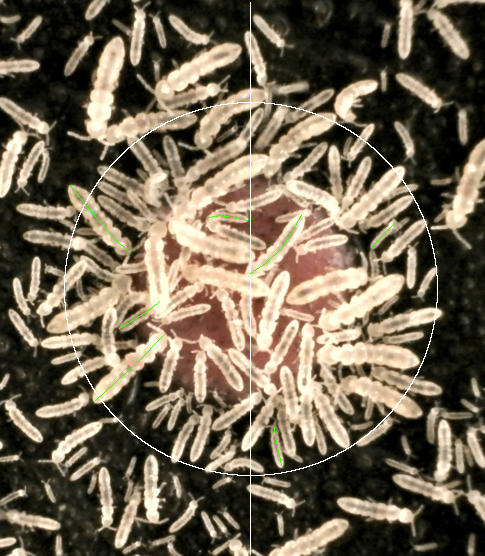
\includegraphics[height=0.25\textheight]{1_CorpsDeThese/Resumes/Fig/SM01b}
\caption[\lofimage{1_CorpsDeThese/Resumes/Fig/SM01}Exemple de comptage
sur une pastille]{Exemple de comptage
sur une pastille, les individus inclus dans le cercle sont comptés,
partiellement ou totalement à gauche, totalement uniquement à droite. Les
lignes vertes montrent le comptage et la mesure de quelques individus.}
\label{fig:SM1b}
\end{center}
\end{figure}

Les séries de photographies récoltées permettent de mesurer la taille des
individus accédant à la ressource à 10 moments que l'on considère indépendants.
L'ensemble des individus accédant à la ressource est mesuré à la main à l'aide
du logiciel d'analyse d'image ImageJ (Figure \ref{fig:SM1b}). Sur chacune des
photos analysées, la pastille est coupée verticalement en deux. Sur une des moitiés, l'ensemble des
individus en contact avec la pastille sont comptés, qu'ils soient partiellement
ou intégralement sur la pastille. Sur la seconde moitié, seuls les individus
intégralement sur la pastille sont mesurés. Ainsi on obtient dix distributions
de la taille des individus accédant à la ressource, dont on compare la moyenne à
la distribution de la taille dans la population totale.

\subsubsection{Mesure du biais d'accès aux ressources}

La distribution de la taille des individus accédant à la ressource comparée à
celle dans la population totale nous permet de mesurer un biais de taille
corporelle dans l'accès aux ressources.

\begin{figure}[!ht]
\begin{center}
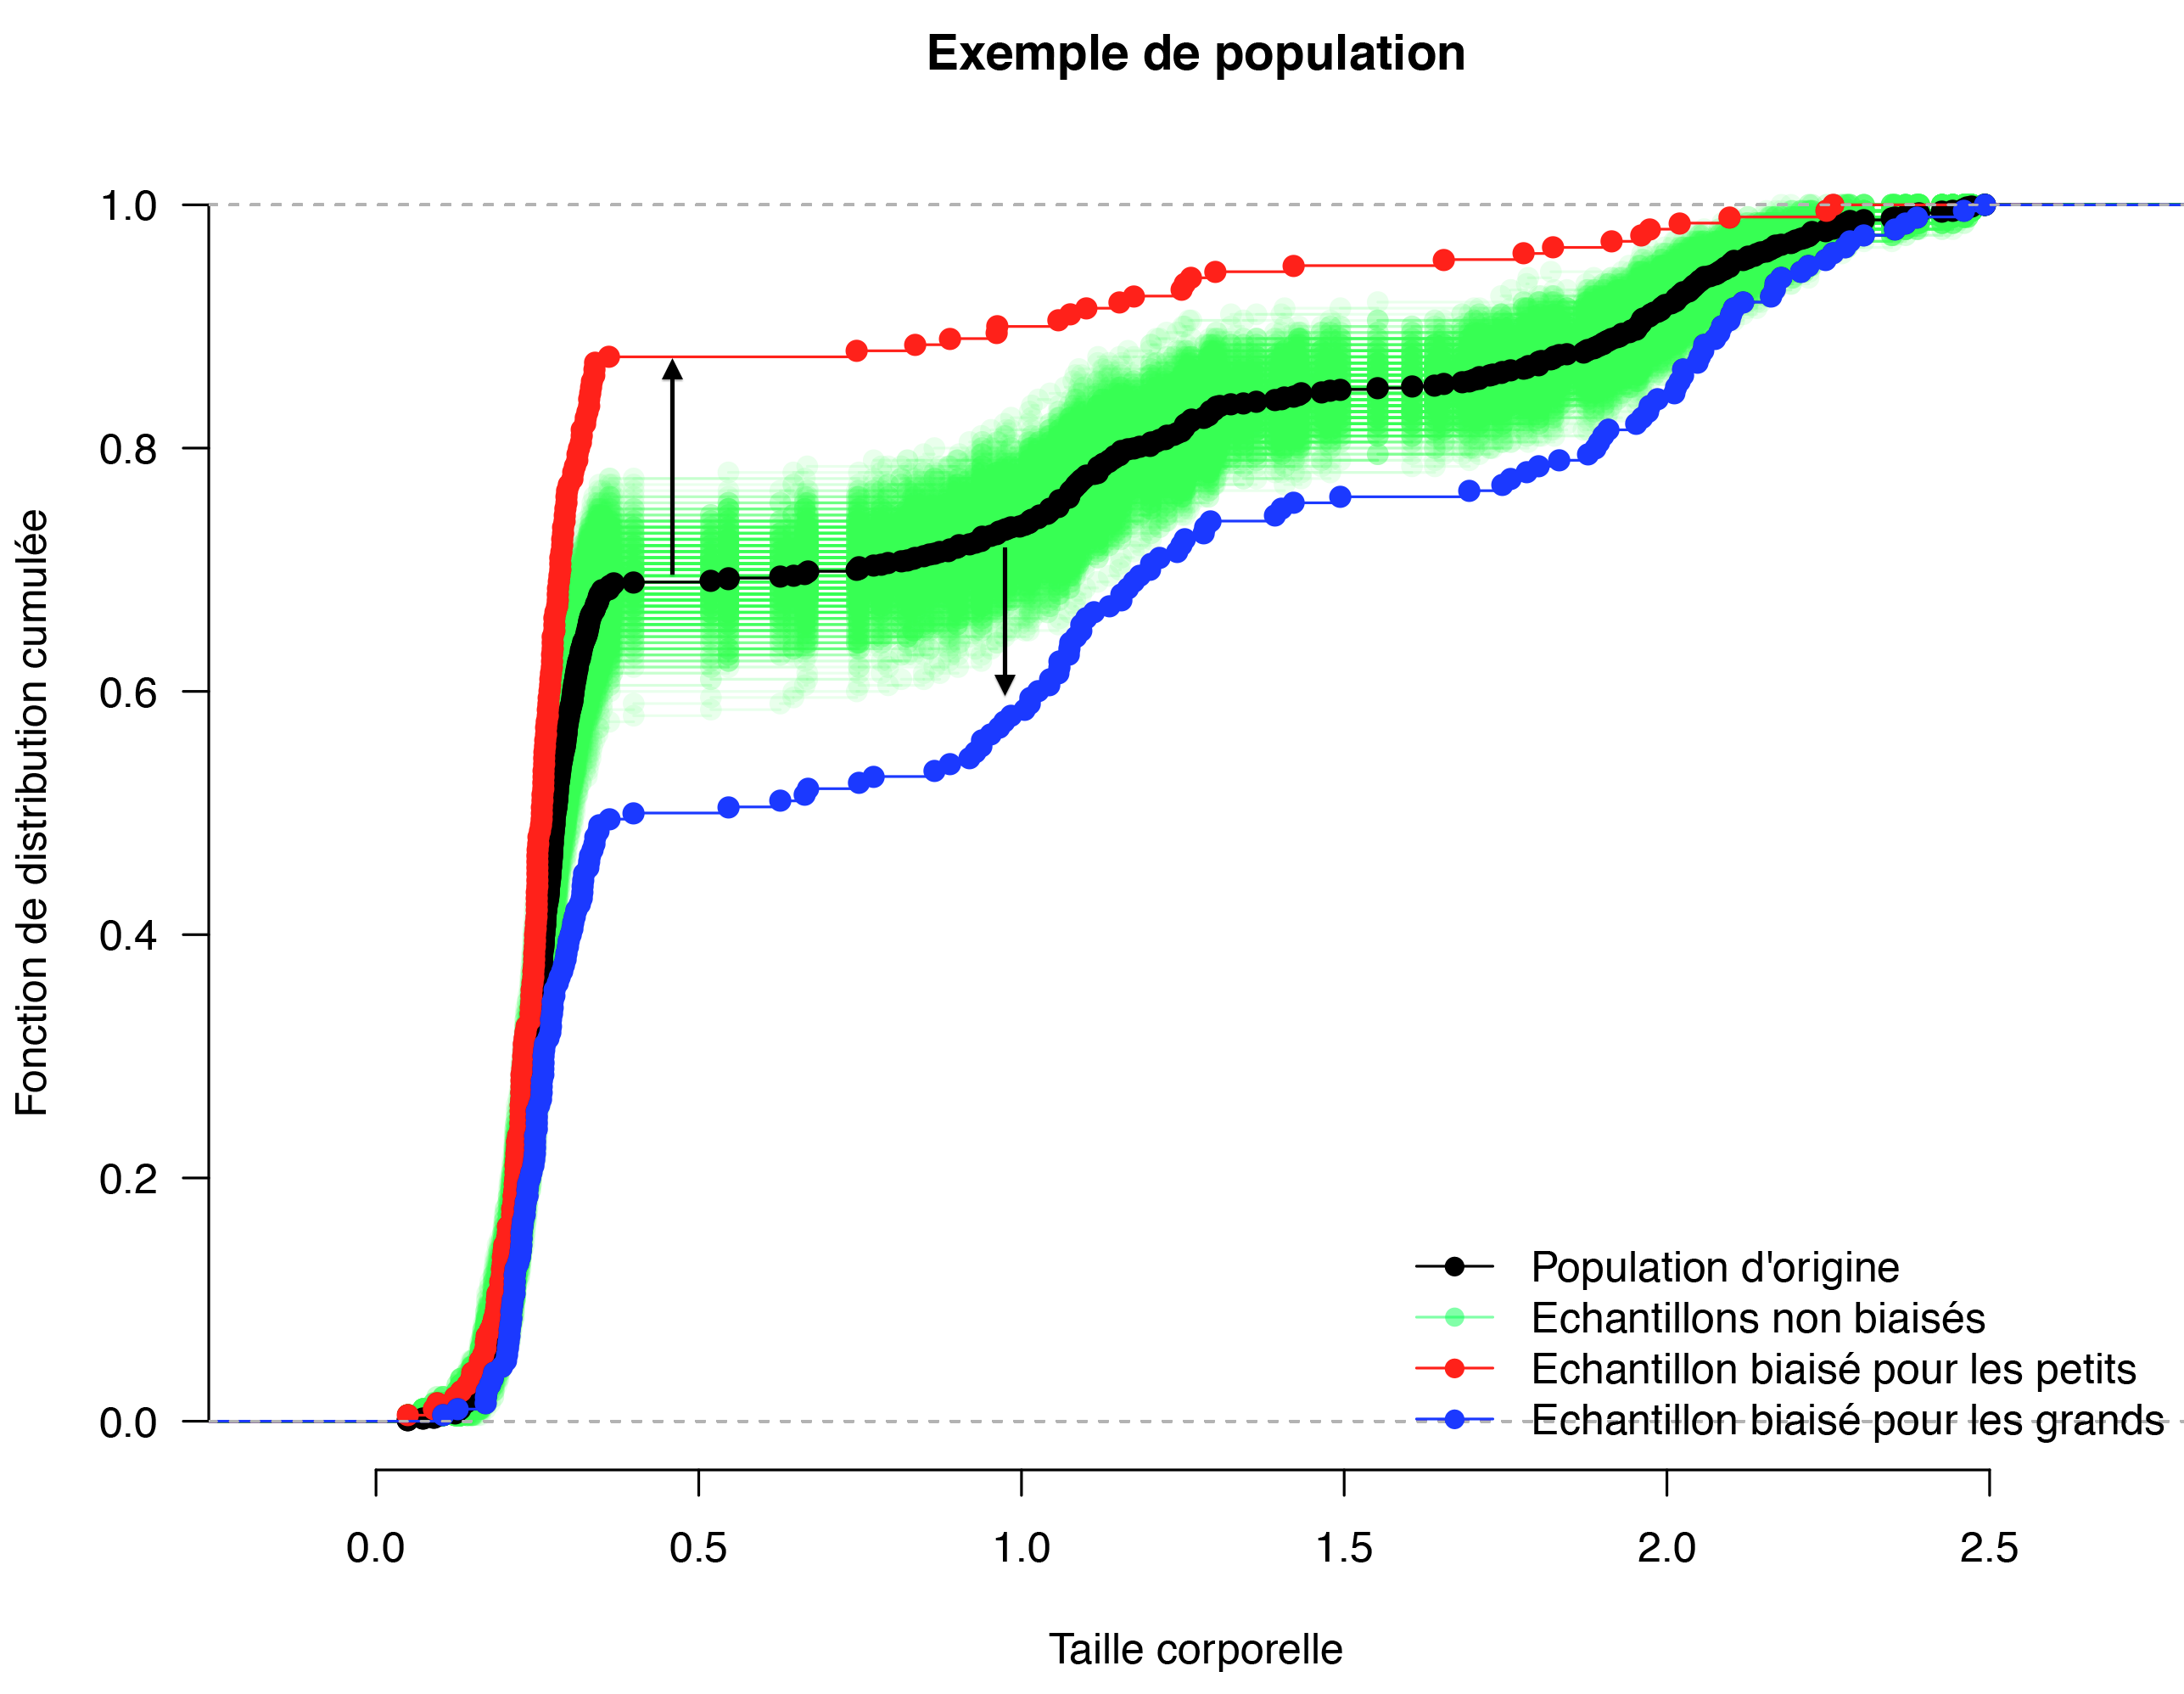
\includegraphics[width=0.66\textwidth]{1_CorpsDeThese/Resumes/Fig/SM02}
\caption[\lofimage{1_CorpsDeThese/Resumes/Fig/SM02}Comparaison des
distributions cumulées]{Exemple de comparaison des distributions cumulées entre
une population totale hypothétique (890 individus) et différents échantillons de
cette population (200 individus).
}
\label{fig:SM2}
\end{center}
\end{figure}

Les différences de distribution en taille des individus qui accèdent à la
ressource sont mesurées et comparées à la population originale en comparant les
fonctions de distribution cumulées de la taille (Figure \ref{fig:SM2}). Nous
utilisons les tests de Kolmogorov-Smirnov (KS) à deux échantillons afin de
tester la significativité de la différence et sa direction. Si la distribution cumulée
de la taille des individus accédant à la pastille est au-dessus de celle de la
population totale, cela signifie qu'il y a en proportion d'avantage de petits
individus accédant à la pastille de ressource que dans la population totale
(Figure \ref{fig:SM2}, échantillon rouge). A l'inverse, si la fonction de
distribution cumulée de la taille des individus accédant à la pastille est en
dessous de celle dans la population totale, cela signifie qu'en proportion, plus
d'individus de grande taille se trouvent sur la ressource que dans la population
totale (Figure \ref{fig:SM2}, échantillon bleu).

Les individus qui accèdent à la ressource représentent un sous-échantillon de la
population totale. Même si le test KS est significatif, nous avons vérifié que
cet échantillon est significativement différent d'un échantillon de même taille
tiré aléatoirement dans la population. Pour chaque population observée, nous
avons tiré aléatoirement $1000$ échantillons de même taille que celui des
individus accédant aux ressources afin de créer un intervalle de confiance des
échantillons aléatoires de la population totale (Figure \ref{fig:SM2},
échantillons verts). Si la distribution des individus accédant aux ressources
est en dehors de cet intervalle, cela confirme que le biais mesuré par le test KS
n'est pas dû au hasard.

% Afin d'avoir une mesure de ce biais et de sa direction, nous comparons la
% distance entre la distribution cumulée de la taille dans la population d'origine
% et la distribution moyenne de la taille des individus accédant à la ressource.
% La distance est calculée comme étant l'aire entre les deux courbes. La distance
% est soit absolue, il s'agit alors simplement de la mesure de l'aire entre les
% deux courbes, soit relative, il s'agit alors d'une aire positive si la
% distribution de l'échantillon est au dessus de celle de la distribution
% d'origine, négative si elle est en dessous. On peut alors tracer sur un graphe
% la distance relative en fonction de la distance absolue (\ref{fig:SM2}b). La
% position du point donne une indication de la direction et de l'intensité du
% biais.



\section{Résultats}

\subsection{Manipulation de la structure}

Les diagrammes structure-temps des populations témoins sont montrés figure
\ref{fig:SM3} et les populations manipulées sont présentées sur la Figure
\ref{fig:SM4}.

\begin{figure}[!ht]
\begin{center}
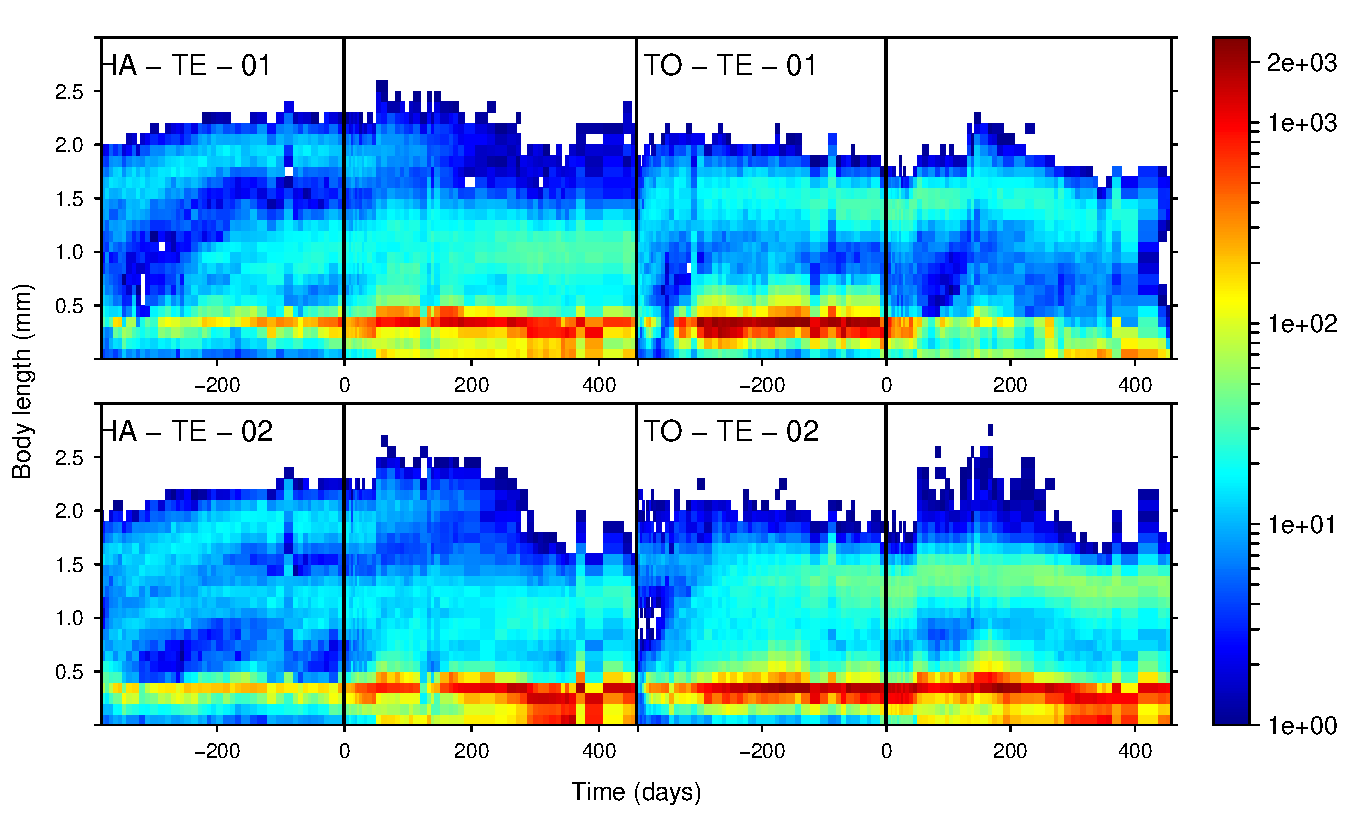
\includegraphics[width=1\textwidth]{1_CorpsDeThese/Resumes/Fig/SM04}
\caption[\lofimage{1_CorpsDeThese/Resumes/Fig/SM04}Population
témoins des clones HA et TO]{Population
témoins des clones HA et TO. La ligne vertical à la date 0 marque le moment où
les populations ont été manipulées.}
\label{fig:SM3}
\end{center}
\end{figure}

Dans les populations témoins, on constate que le changement de boite d'élevage
n'a pas eu d'effet immédiat sur les dynamiques des structures de populations. En
effet, on ne remarque pas de changement abrupt dans la structure de la
population au moment du transfert. Au contraire, les dynamiques observées
peuvent être comparées aux dynamiques présentées dans les Chapitre \ref{chap:sp}
(voir aussi Annexe \ref{Ann:SP}). Chez le clone HA, les deux populations témoins
sont trimodales au moment du transfert de boite d'élevage. Il semble que dans
les deux boites le mode des adultes les plus grands soit déjà décroissant au
moment du transfert et il s'éteint quelque temps après. Le temps de survie de ce
mode dans chacune des populations est de l'ordre de 500 jours, ce qui correspond
aux durées observées dans les populations non manipulées du Chapitre
\ref{chap:sp} (voir aussi Annexe \ref{Ann:SP}). Les deux populations TO montrent
également des dynamiques similaires aux populations non manipulées. On ne
constate pas de modification majeure dans la dynamique suite au transfert des
populations dans une nouvelle boite d'élevage.

\subsubsection{Traitements 1: Je - MG}

Dans ce traitement, la classe des juvéniles (Je) est isolée dans une boite alors
que les petits et grands adultes sont conservés ensemble et placés également
dans une nouvelle boite. Que ce soit pour le clone HA ou TO, on constate dans
les populations de juvéniles isolés le démarrage de la croissance d'une grande
partie des juvéniles dès le jour 0 (jour du transfert). Les ressources étant
apportées dans la même quantité qu'avant la manipulation, on observe l'effet du
relâchement de la compétition qui donne la possibilité aux juvéniles de grandir.
La cohorte qui démarre une croissance est très dense et conduit la structure de
la population vers une structure de type 1 (Chapitre \ref{chap:sp} et Annexe
\ref{Ann:SP}) avec des petits adultes en grande quantité et un grand nombre de
juvéniles. Dans ce traitement, les dynamiques des clones HA et TO sont très
semblables. En effet, le nombre de juvéniles qui maturent d'un coup est
suffisamment important pour empêcher HA d'exprimer sa capacité à produire des
adultes de grande taille.

\afterpage{%
    \clearpage% flush all other floats
    \ifodd\value{page}
    %\else% uncomment this else to get odd/even instead of even/odd
        \expandafter\afterpage% put it on the next page if this one is odd
    \fi
    {%
    \begin{figure}[p]
        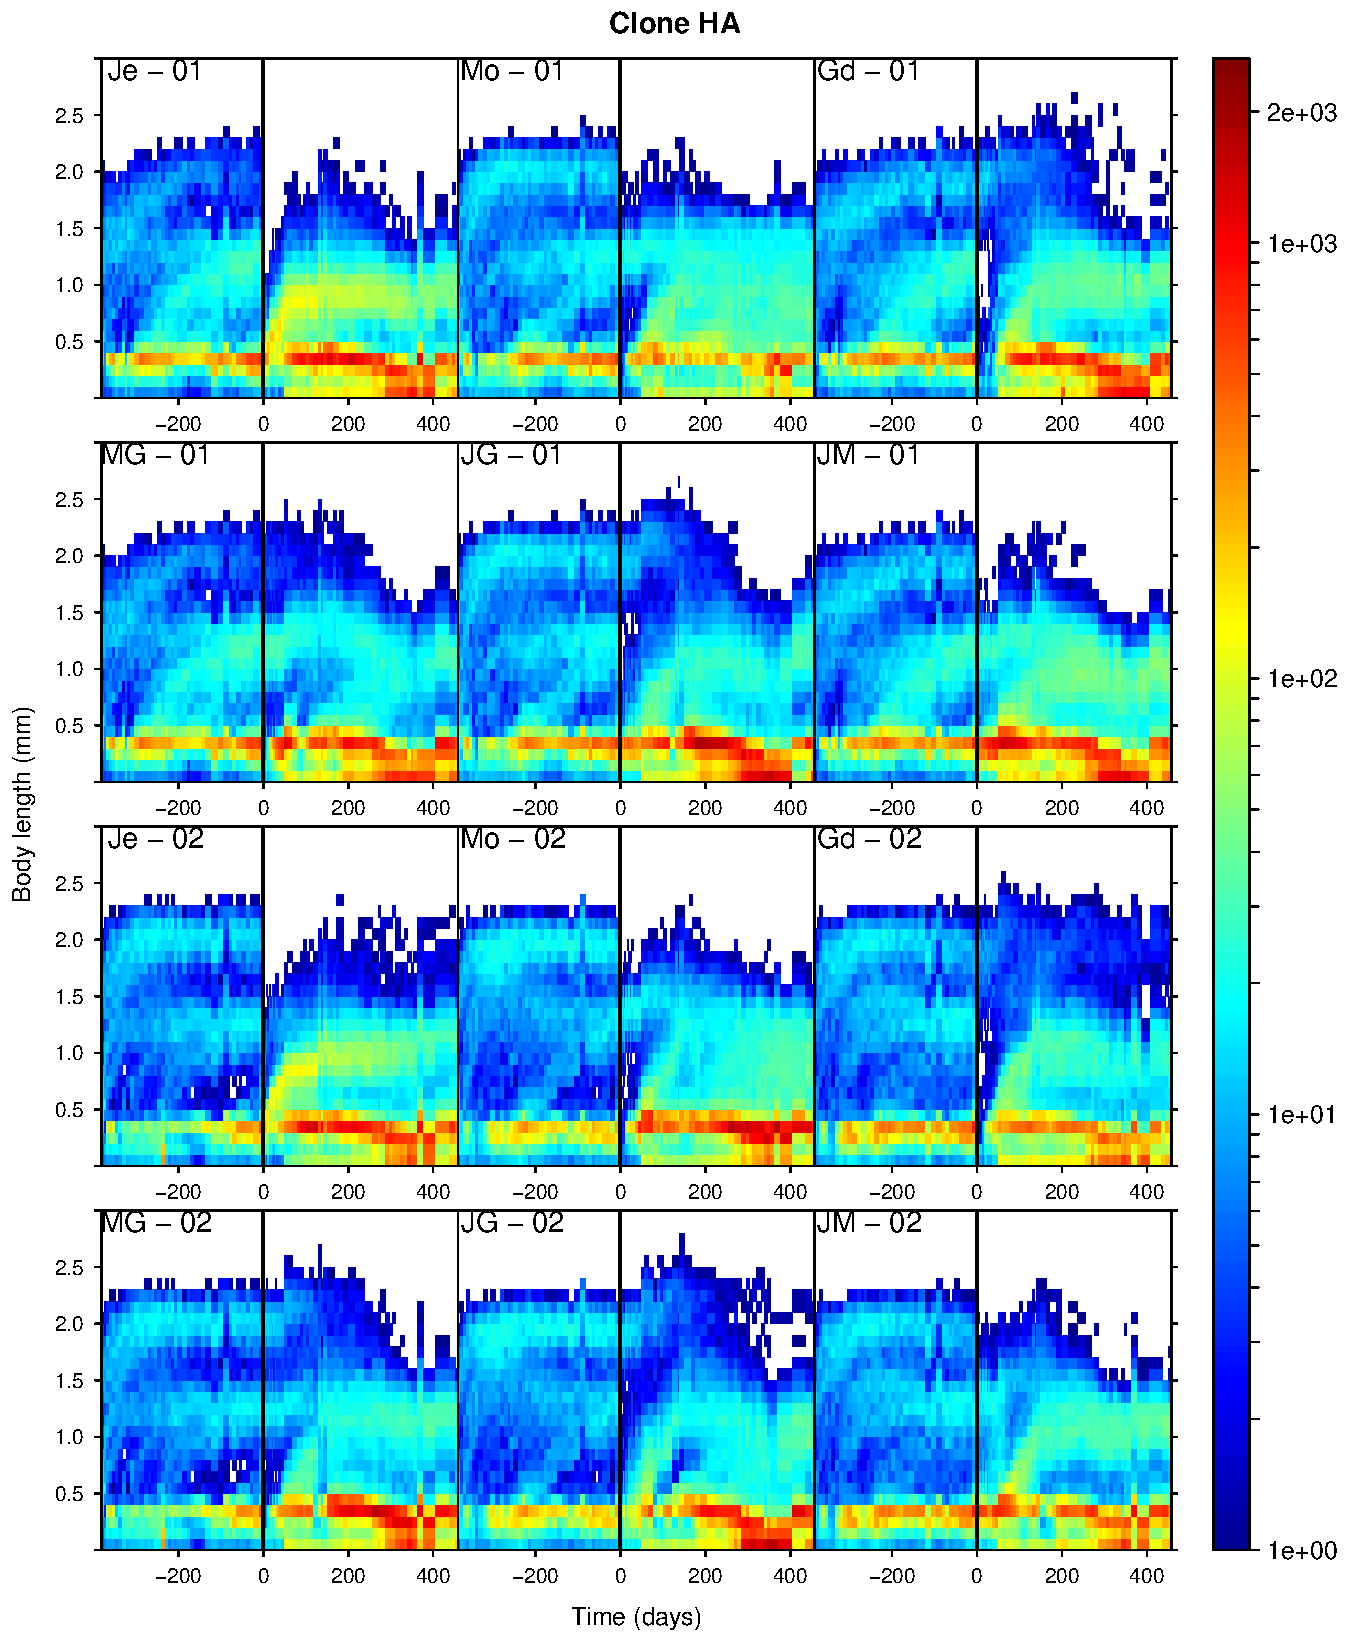
\includegraphics[width=\textwidth]{1_CorpsDeThese/Resumes/Fig/SM03a}
        \caption[\lofimage{1_CorpsDeThese/Resumes/Fig/SM03a}Diagrammes
        structure-temps des populations manipulées]{Diagrammes
        structure-temps des populations manipulées. La ligne vertical à la date 0 marque le moment où les populations ont été
        manipulées. Clone HA\ldots}\label{fig:SM4}
    \end{figure}
    \clearpage
    \begin{figure}[p]
		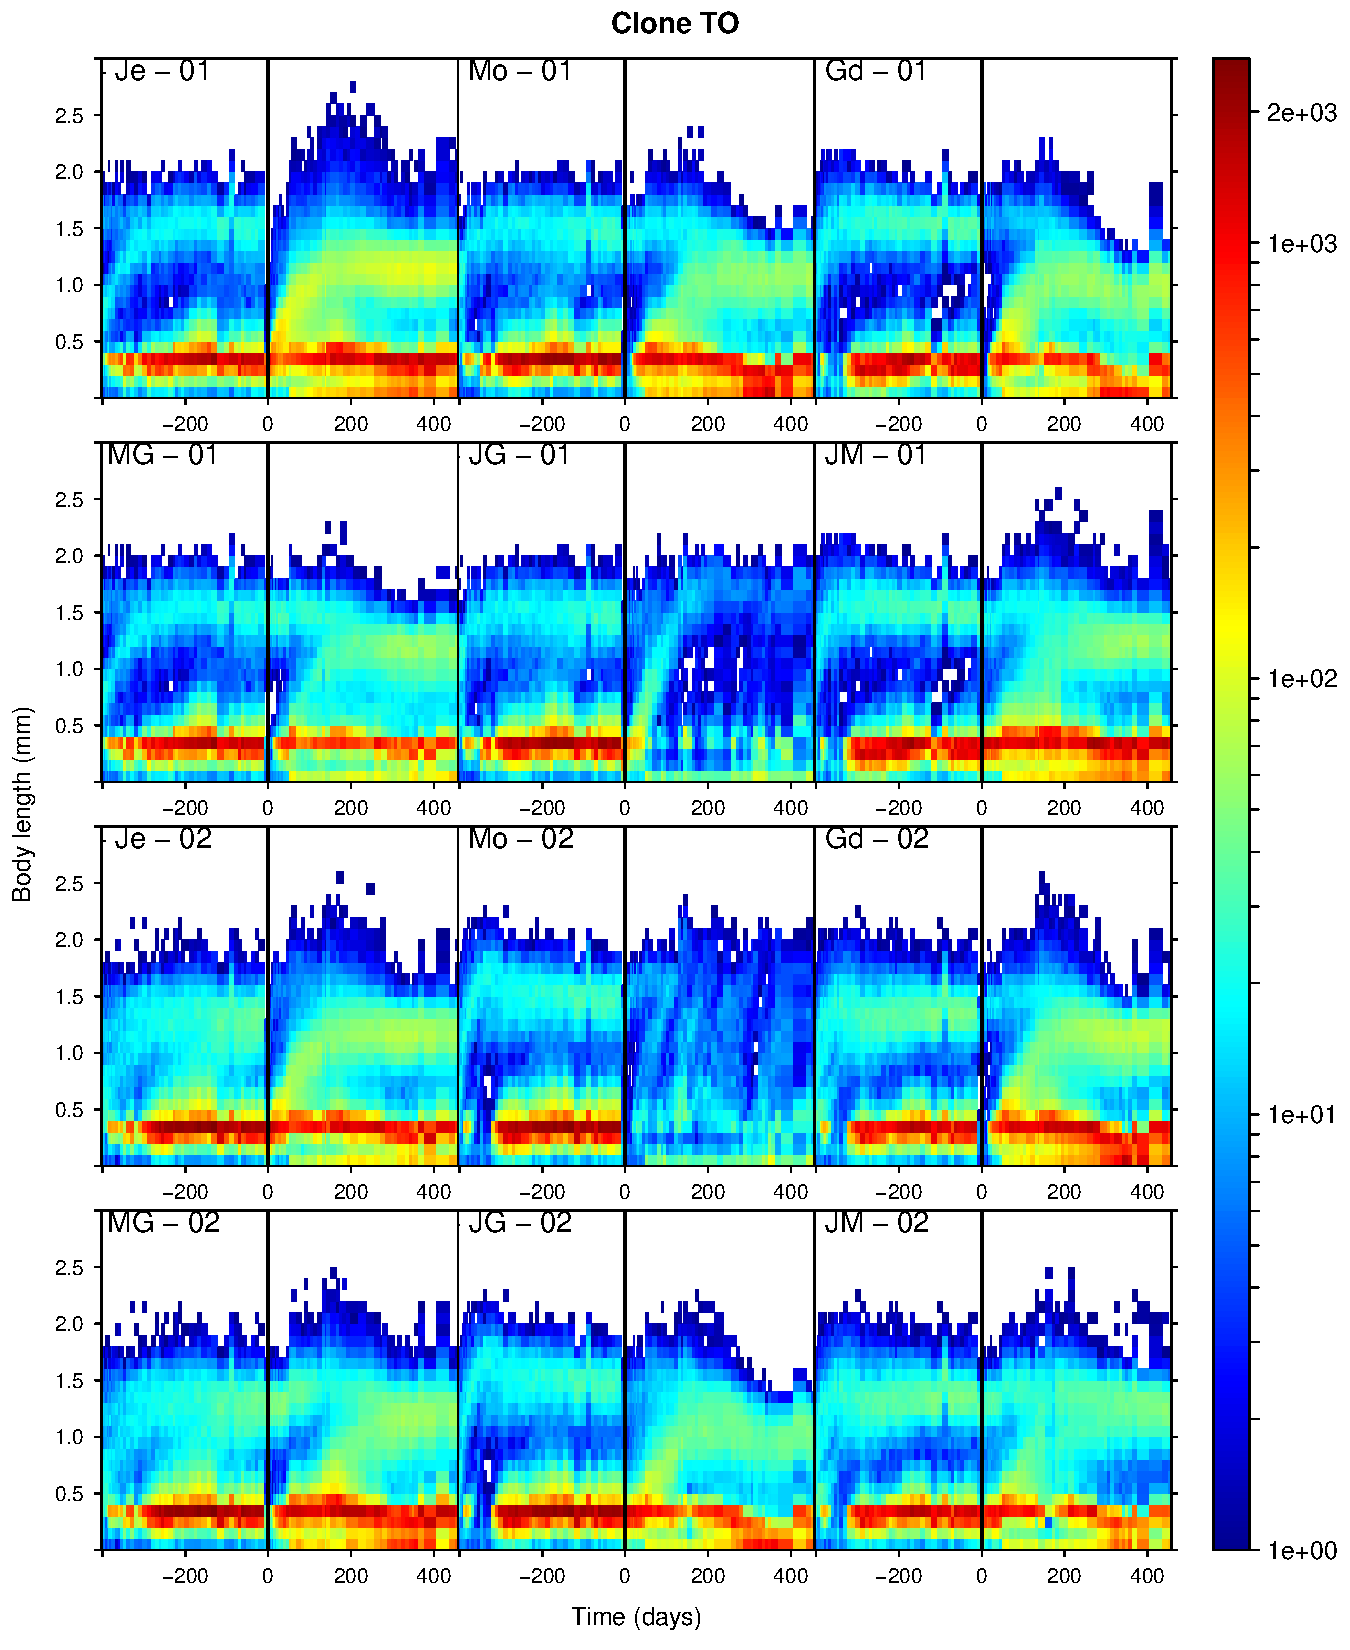
\includegraphics[width=\textwidth]{1_CorpsDeThese/Resumes/Fig/SM03b}
        \caption*{\ldots et Clone TO.}
    \end{figure}
    \clearpage
    }%
}



Dans les populations des adultes (MG), on constate chez HA que dès la
séparation les adultes reprennent également de la croissance. Ceci coïncide
également avec une disparition de la cohorte des adultes les plus grands. Cette
reprise de croissance semble montrer que malgré leurs faibles capacités
d'interférence, les juvéniles, de part leur grand nombre, exerce quand même une
pression de compétition par exploitation sur les adultes, limitant leur
possibilité de croissance. D'un point de vue de la dynamique de la structure,
dès la séparation, les adultes ont pondu et de nouvelles éclosions surviennent
après quelques semaines. On se retrouve alors de nouveau dans une situation
proche des structures de type 1 (Chapitre \ref{chap:sp} et Annexe \ref{Ann:SP}).
Ainsi, malgré le relâchement de la compétition par exploitation, les adultes les plus grands finissent par s'éteindre comme
dans les populations témoins, et ne sont pas remplacés. 

Chez le clone TO, la situation est similaire, avec un léger ajustement de la
taille immédiatement après la séparation de la population. Mais cet ajustement
s'accompagne de ponte très importantes et de nombreuses éclosions suivies de
la croissance d'une cohorte qui ramènent de nouveau les populations vers une
structure composée de petits adultes et d'un grand nombre de juvéniles.
Ainsi, le retrait des juvéniles n'a que peu d'effet car les adultes renouvellent très rapidement le
pool de juvéniles grâce à leur grande capacité de ponte. En quelques semaines,
les populations ont absorbé la perturbation et la dynamique semble peu affectée.
Il semble que ce soient les adultes de la population qui soient
responsable de la résilience de sa structure en taille: le retrait des juvéniles
modifie peu la dynamique de la structure, alors que le retrait de l'ensemble des
adultes a un effet important sur cette dynamique et peut faire basculer entre
différents types de structure. 

\subsubsection{Traitements 2: Mo - JG}

Dans ce traitement, les adultes de taille intermédiaire (Mo) sont isolés et les
juvéniles et les grands adultes (JG) sont conservés ensembles.

Chez les deux clones, l'isolation des adultes moyens (clone HA) ou de deux tiers
des adultes (clone TO) provoque une légère reprise de croissance accompagnée de
larges pontes et de la croissance d'une cohorte, qui ramène les populations dans
une structure semblable au traitement MG. Encore une fois, le retrait d'une
partie de la population relâche la compétition, ce qui explique la reprise de croissance,
mais celle-ci n'est pas suffisante comparée à la croissance des juvéniles pour
que les adultes HA atteignent les tailles du groupe de géant, ce qui ne permet
pas aux populations HA de retrouver une structure trimodale. Chez TO, la
deuxième population (TO Mo - 02) présente une réponse différente à la
perturbation. Lors du transfert des adultes moyens dans une nouvelle boite, il
semblerait qu'il y ait eu une forte mortalité et la population entre dans une
sorte de période cyclique avec des recrutements et remplacement des adultes
successifs. Ceci s'apparente d'avantage à une situation où les plus petits
individus dominent la population, ce qui pourrait s'expliquer par l'éclosion
rapide d'un grand nombre de juvéniles alors que peu d'adultes sont présents. 

Dans les populations JG, on constate là encore une reprise de croissance chez
les adultes restant, et des éclosions massives peu de temps après la séparation.
Chez HA, les adultes de grande taille meurent peu à peu et les populations
retournent à une distribution bimodale. Chez TO, on observe là encore deux cas
différents, dans le premier, une cohorte de petite densité parvient à grandir
jusqu'à une taille relativement importante, il y a alors relativement peu de
pontes, et la population se maintient avec une structure de type 2 (Chapitre
\ref{chap:sp} et Annexe \ref{Ann:SP}), alors que dans le second cas, on observe le
comportement classique avec un recrutement massif d'individus, et une population qui converge
vers une structure de type 1.

Ainsi, alors que le retrait des juvéniles avait relativement peu d'effet sur la
structure des populations comparé aux populations témoins, le retrait des
adultes de taille intermédiaire provoque une période transitoire un peu plus
longue qu'au par avant, voir un changement d'attracteur et la convergence vers
une structure et une dynamique très différente. 

\subsubsection{Traitements 3: Gd - JM}

Dans ce traitement, les juvéniles et les adultes de petite taille (clone HA) ou
les deux tiers des adultes (clone TO) sont conservés ensemble, le reste des
adultes (les grands pour HA et le tiers restant pour TO) est isolé. 

Dans les populations de grands adultes isolés (Gd), la réponse à la perturbation
est similaire à ce qui était observé pour les populations d'adultes
intermédiaires (Mo). En effet, la séparation des populations est suivie par une
période transitoire où les adultes restant grandissent légèrement et produisent
de nouvelles pontes. Lorsque ces pontes éclosent, une cohorte recrute
directement chez les adultes intermédiaires mais pas chez les plus grands. De
même pour TO, des cohortes très denses recrutent et atteignent rapidement la
taille adulte. 

Il est plus intéressant de noter que le retrait des adultes les plus grands des
populations HA  (JM 01 et 02) provoque également le recrutement d'une nouvelle
cohorte, mais plus dense que dans les traitements JG (où les adultes
intermédiaires sont retirés). Ainsi, bien que l'on retire moins d'individus
de la population (la cohorte d'adultes de grande taille est moins dense), le
fait de retirer les individus les plus grands des populations HA permet un
recrutement plus massif chez les juvéniles, ce qui signifie que la compétition
pour la ressource est retombé à un niveau plus bas que pour les traitements JG.
Chez TO, on n'observe pas ce phénomène car les traitements JM et JG diffèrent
par le nombre d'individus retirés des populations mais pas par la taille des
individus. Ainsi, en retirant le groupe G, on retire deux fois moins d'individus
que dans le groupe M, mais de la même taille. L'effet sur la compétition est
donc d'avantage lié au nombre d'individus retirés, plus qu'à la taille de ces
derniers. 

\subsubsection{En résumé}

Ces différents traitements semblent montrer que la présence d'adultes dans la
population affecte directement la capacité des juvéniles à grandir et arriver
à maturation. En effet, dès la suppression d'une partie des adultes, les
juvéniles présents dans la population se mettent immédiatement à grandir, et si
aucun juvénile n'est présent, les nouveaux nés démarrent également leur
croissance immédiatement. Cet effet des adultes sur la dynamique de la structure
des populations se manifeste au travers de deux facteurs, leur nombre et leur
taille. Si tous les adultes sont de même taille, le retrait d'une plus grande
quantité d'adultes permet à un plus grand nombre de juvéniles de recruter. Mais
ce qui est plus intéressant, c'est que si des adultes de taille différentes sont
présents, le retrait des adultes les plus grands, même s'ils sont moins nombreux
permet à d'avantage de juvéniles de grandir. Cela montre que la taille des
adultes joue un rôle direct sur la pression de compétition qu'ils imposent aux
juvéniles, ce qui est un argument qui soutient la compétition par
interférence comme mécanisme de régulation de la dynamique. 

\subsection{Observations comportementales}

Dans un second temps, nous nous sommes intéressés aux comportements
individuels d'accès à la ressource disponible. Les observations ont été
réalisées sur certaines des populations manipulées dans l'expérience précédente.
Ces observations comportementales et la mesure du biais de taille dans la capacité à accéder aux
ressources va nous permettre de confirmer le rôle de la compétition par
interférence.

\subsubsection{Exemple d'observation comportementale}

\begin{figure}[!ht]
\begin{center}
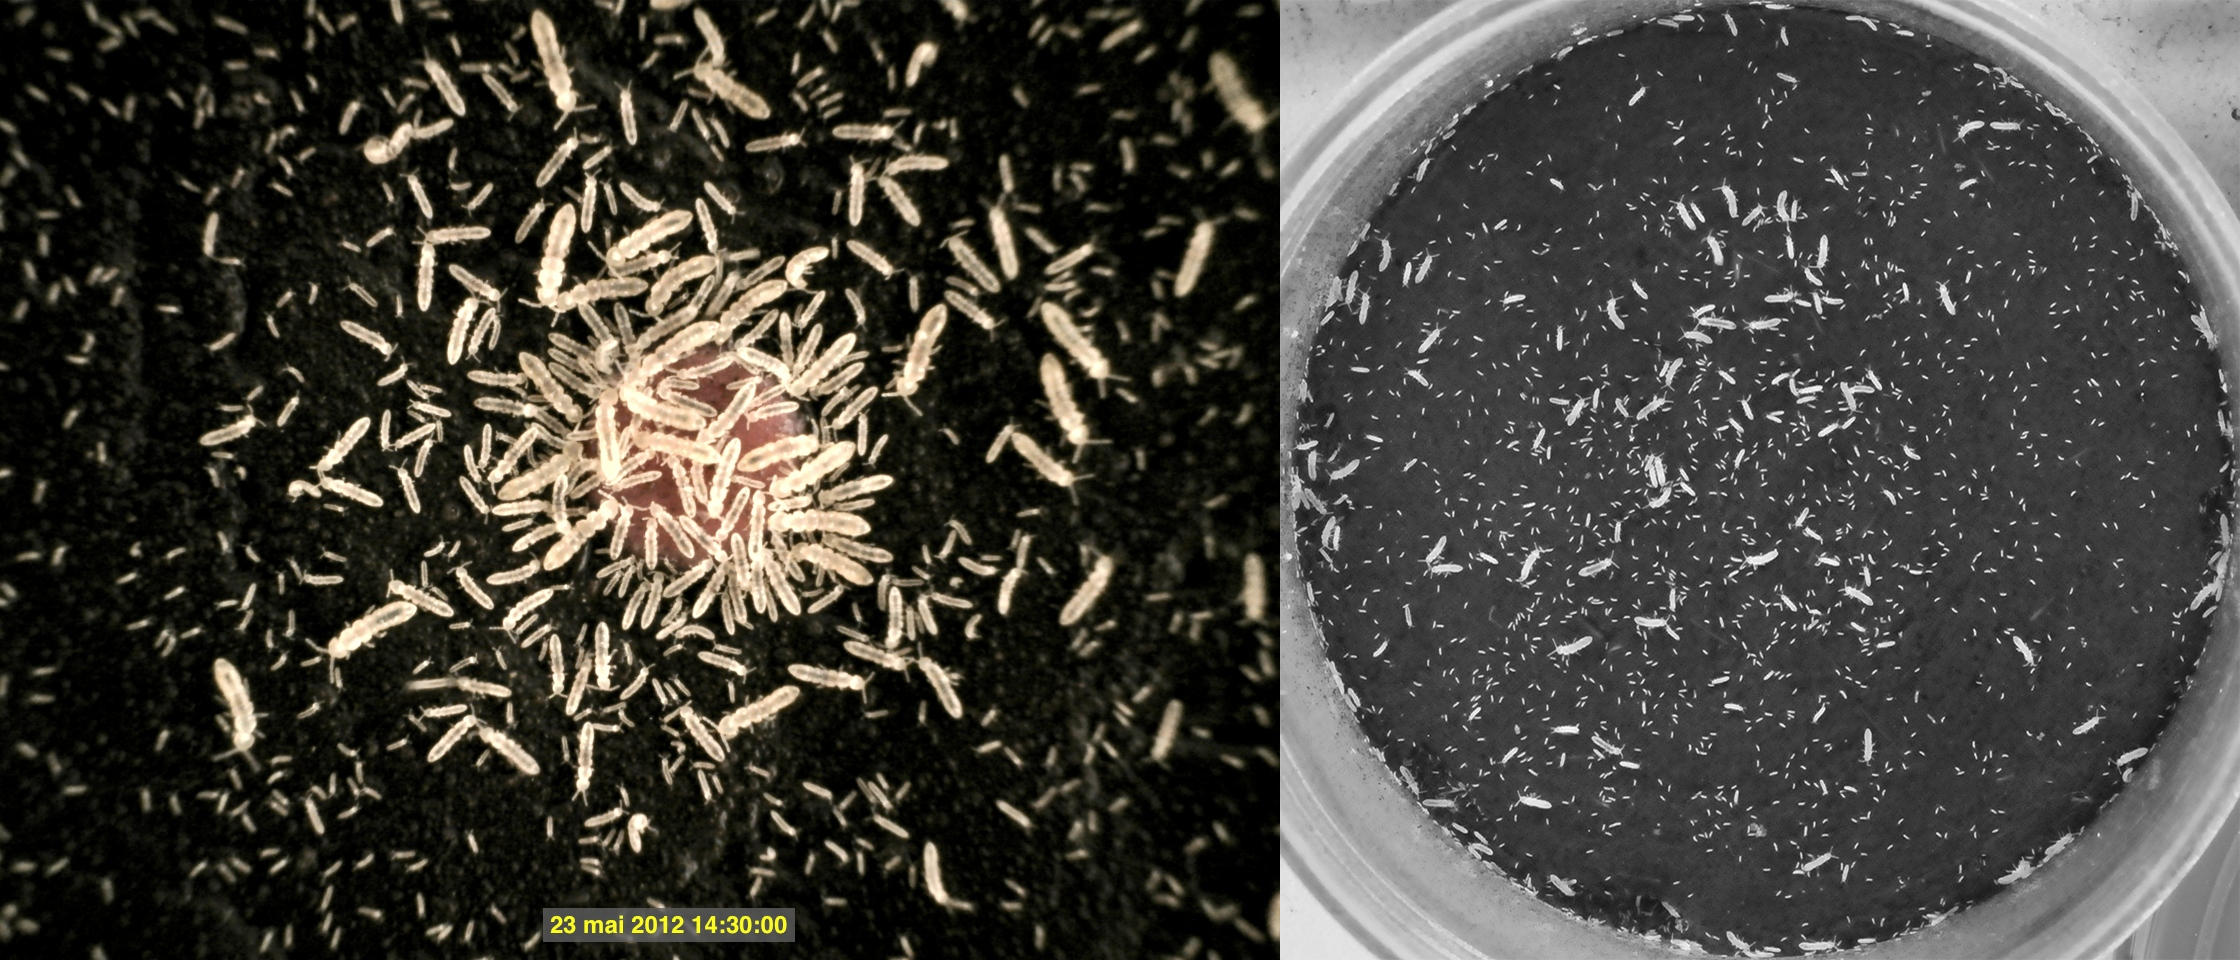
\includegraphics[width=1\textwidth]{1_CorpsDeThese/Resumes/Fig/SM05b}
\caption[\lofimage{1_CorpsDeThese/Resumes/Fig/SM05b}Cliché
d'observation de l'accès à la ressource]{Cliché
d'observation de l'accès à la ressource pour la population témoin HA-01 et
cliché de la population totale à une date proche.}
\label{fig:SM5}
\end{center}
\end{figure}

La Figure \ref{fig:SM5} montre un exemple de cliché pris au cours de
l'observation comportementale de l'accès aux ressources. Ce cliché a été pris
pour la population témoin HA 01. Bien que ce ne soit qu'un seul exemple de
cliché, cet exemple est très représentatif de ce qui a été observé dans toutes
les populations mesurées. On peut observer sur ce cliché une forte concentration
d'individus regroupés sur la pastille de nourriture (en rouge au centre) et des
individus plus dispersés aux alentours. Il est intéressant de constater la
différence de taille des individus sur ou aux abords de la pastille de ressource
comparée à la celle des individus plus éloignés et à l'ensemble des individus de
la population. Alors que les individus éloignés sont majoritairement des
juvéniles, les individus les plus gros présents sur ce cliché sont tous sur la
pastille de ressource ou dans ses environs proches.
Ceci est observé alors même qu'en nombre d'individus, cette population est
largement dominée par les juvéniles. Si l'accès à la ressource était indépendant
de la taille, on s'attendrait donc à avoir davantage de juvéniles présents sur
la pastille que de grands individus. Il y a donc un biais de taille corporel
manifeste dans l'accès à la ressource.

\begin{figure}[!ht]
\begin{center}
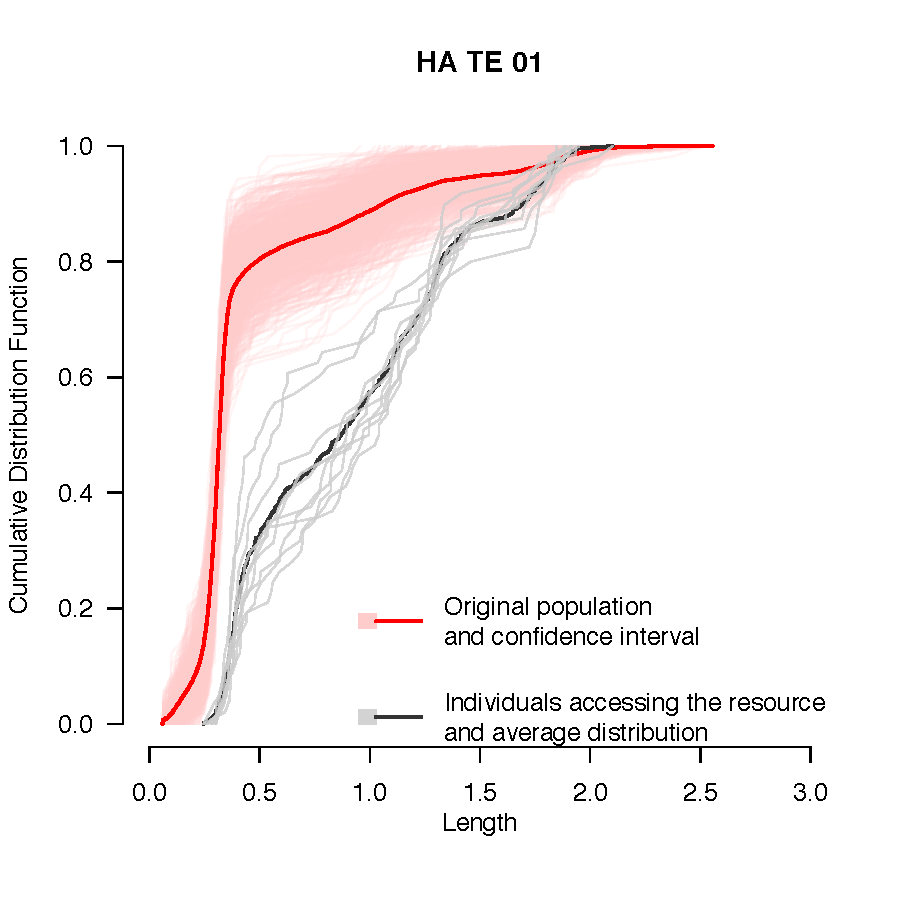
\includegraphics[width=0.75\textwidth]{1_CorpsDeThese/Resumes/Fig/SM06}
\caption[\lofimage{1_CorpsDeThese/Resumes/Fig/SM06}Mesure du biais
d'accès aux ressources]{Mesure du biais
d'accès aux ressources pour la population témoin HA 01. Test de
Kolmogorov-Smirnov de comparaison de deux échantillons: gris en dessous du
rouge: $p<10^{-10}$.}
\label{fig:SM6}
\end{center}
\end{figure}

Le cliché présenté en Figure \ref{fig:SM5} fait partie d'une série de 10 clichés
de la même population à 15 minutes d'intervalle. La Figure \ref{fig:SM6}
présente les fonctions de distribution cumulées de la population totale (rouge),
des individus accédant à la ressource sur chacun des clichés (gris clair), de la
moyenne des individus accédant à la ressource (gris foncé), et de 1000
échantillons aléatoires de même taille que la distribution moyenne des individus
accédant à la ressource (rouge clair). On constate que les dix distributions en
gris sont systématiquement en dessous de la distribution dans la population entière. Qui
plus est, elles sont également systématiquement en dehors de l'intervalle des
sous échantillons aléatoires. Le test de comparaison des distributions,
effectué avec la distribution moyenne sur la pastille est également extrêmement
significatif.
Cela nous permet d'affirmer qu'il y a un biais significatif en faveur des
individus les plus grands de la population dans l'accès à la ressource. En
effet, alors que $80\%$ des individus de la population mesurent moins de
$0.5mm$, ils ne représentent qu'un tiers des individus présents sur ou aux
abords de la pastille de nourriture. De plus, $13\%$ des individus sur la
ressource mesurent plus de $1.6mm$ alors qu'ils représentent moins de $5\%$ de
la population totale. Enfin, $50\%$ des individus présents sur la pastille ont
une taille entre $0.45$ et $1.35mm$ alors que cette classe de taille ne
constitue que $15\%$ de la population totale.

\subsubsection{Mesure du biais d'accès aux ressources}

La mesure du biais par comparaison des distributions cumulées a été réalisée sur
10 populations. La Figure \ref{fig:SM7} présente les distributions cumulées des
neufs autres séries d'observation.
On constate que dans tous les cas il existe un biais en faveur des individus les
plus grands pour l'accès à la ressource. On constate également que même dans les
populations où le nombre de grands individus est relativement important, telle
que TO TE 01, le biais reste significatif avec une large sous représentation des
$40\%$ d'individus de moins de $0.5mm$.

On remarque encore que même dans les populations où les juvéniles représentent
plus de $80\%$ de la population totale (HA JM 01, HA JM 02, HA TE 02, TO MG 02),
on ne comptabilise sur la ressource jamais plus de $50\%$ d'individus de moins
de $0.6mm$. Sur l'ensemble des cas étudiés, les $10\%$ les plus grands des
individus de la population totale représentent jusqu'à plus de $50\%$ des
individus mesurés sur les ressources, et généralement autour de$20\%$.

\begin{figure}[!ht]
\begin{center}
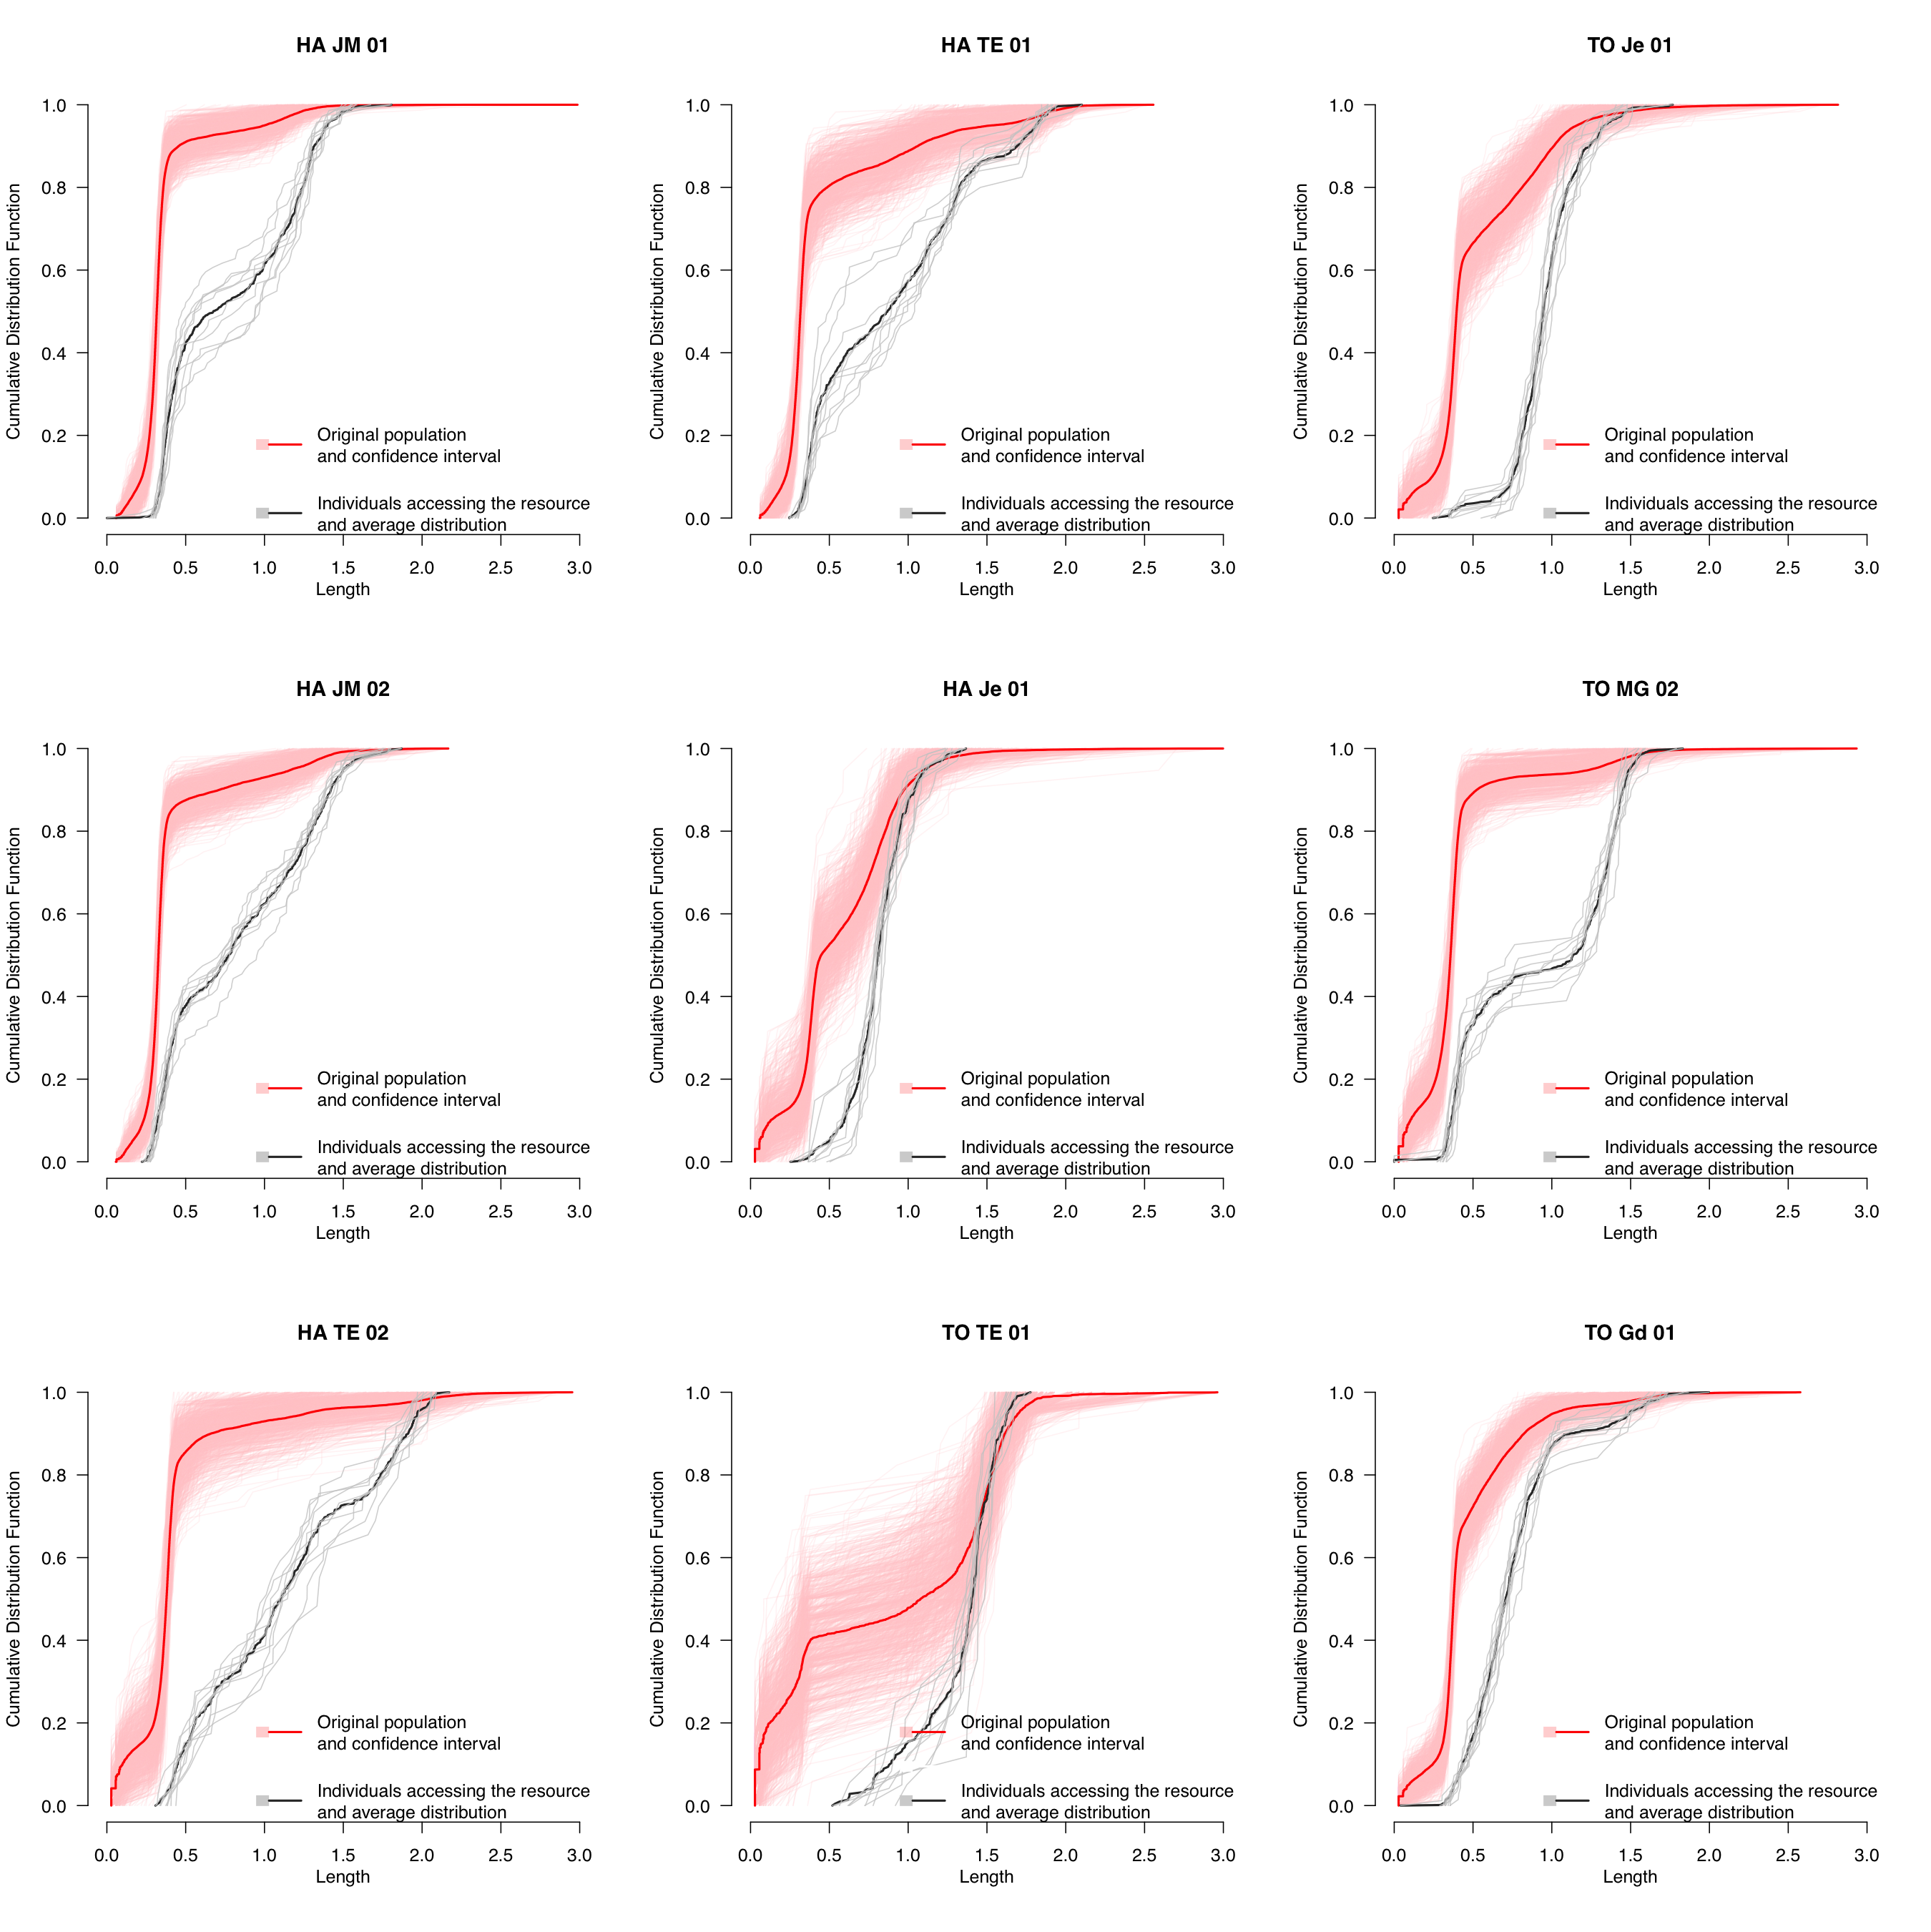
\includegraphics[width=1\textwidth]{1_CorpsDeThese/Resumes/Fig/SM07}
\caption[\lofimage{1_CorpsDeThese/Resumes/Fig/SM07}Mesures du biais
d'accès aux ressources]{Mesures du biais
d'accès aux ressources pour 9 autres populations. Tests KS: $p \ll 0.01$}
\label{fig:SM7}
\end{center}
\end{figure}

Les biais en faveur des grands individus dans l'accès à la ressource semblent
donc être systématiques, quelle que soit la population étudiée. Nous avons
utilisé dans ces observations des populations dont la structuration en taille était
différente.
Ainsi, même avec très peu de grands individus dans la population, ceux-ci sont
très largement sur-représentés lors des comptages sur les pastilles. Il semble
donc que la capacité des individus de grande taille à dominer la ressource soit
commune à nos deux clones, et ne dépende que peu des conditions de densité de la
population. Lors de la prise des clichés servant de base à ces mesures, nous
avons également pu identifier en temps réel des interactions
compétitives entre individus: des individus se
mettaient à tourner rapidement en rond lorsque d'autre s'approchaient de trop prêt, provoquant leur fuite. Ces comportements étaient
particulièrement visibles chez les individus les plus grands, faisant fuir
rapidement les plus petits. Ainsi, la
domination des plus grands individus sur la ressource passe notamment par des
comportements consistant à chasser les individus plus faibles de leur
environnement direct, empêchant les fuyards d'accéder à la ressource. Ce
comportement répond à notre définition précédente de la compétition par
interférence (Chapitres \ref{chap:method} et \ref{chap:amnat}, et Annexe
\ref{An:AmNat}).

\section{Discussion}

Au cours de cette étude, nous avons analysé la réponse de la structure en taille
de populations de collemboles à des perturbations. Plusieurs perturbations ont
été appliquées aux deux clones étudiés jusque là, HA et TO. Ces perturbations
ont consisté à manipuler la structure en taille de la population pour observer
l'établissement d'un nouvel équilibre en fonction des nouvelles conditions
imposées. 

Nous avons également réalisé une série d'observations des
comportements individuels d'accès aux ressources. Ces observations nous ont
permis de mettre en évidence un biais systématique dans l'accès à la ressource
en faveur des individus les plus grands de la population. 

\subsection{Stabilité et résilience des différentes structures en taille}

Au cours de la première expérience, nous avons manipulé la structure de
plusieurs populations des clones HA et TO. Les différentes manipulations
réalisées ont permis de tester la stabilité des différents attracteurs décrits
dans le Chapitre \ref{chap:sp}. En effet, les huit populations HA utilisées
dans l'étude étaient toutes dans une structure de type 4 au moment de la
perturbation, alors que les populations TO étaient dans des structures de type 1
ou 2. Nous avions déjà constaté que les structures de type 4 n'étaient stable
que le temps de survie des adultes les plus grands; une fois disparus,
ces derniers n'étaient pas remplacés et les populations convergeaient vers
différentes structures. Ceci est encore confirmé par nos populations HA témoins,
en effet, les adultes les plus grands survivent après le changement de boite
d'élevage mais meurent de vieillesse après quelques centaines de jours (voir
\autocites{mallard2013b} pour plus d'informations sur le vieillissement).
La structure observée subit alors le même type de transition que les populations présentées
dans le Chapitre \ref{chap:sp} (voir aussi Annexe \ref{Ann:SP}). De plus,
lorsque les adultes les plus grands sont retirés des populations, ils ne sont pas remplacés malgré une légère
croissance des adultes de taille intermédiaire. A la place, une cohorte de
juvéniles parvient à grandir et rejoint les adultes intermédiaires, augmentant
la compétition au sein de cette classe, ce qui empêche une croissance vers les
très grandes tailles. Enfin, lorsque l'on enlève les juvéniles ou les adultes
de taille intermédiaire, les plus grands parviennent à se maintenir quelques
temps après perturbation mais ne sont pas remplacés après leur mort. Cette
structure trimodale est donc stable localement, mais le bassin d'attraction est
trop petit pour permettre de l'atteindre, à part dans des conditions très
particulières telles que décrites dans le Chapitre \ref{chap:sp} (voir aussi
Annexe \ref{Ann:SP}).

A l'inverse, la plupart des populations dont la structure a été modifiée au
moment de la manipulation convergent vers une structure avec un grand nombre de
juvéniles, et des adultes plutôt petits et en assez forte densité. Cette
structure, similaire aux structures de type 1, semble donc avoir un bassin
d'attraction plus large que les autres car elle est atteinte quel que soit la
manipulation effectuée sur la structure. Cette structure est généralement
atteinte lorsque beaucoup de juvéniles grandissent et atteignent la maturité en
même temps. Au cours de nos différentes manipulations, soit des juvéniles
étaient présents et pouvaient grandir dès que la pression de compétition était
relâchée par le retrait de tout ou partie des adultes, soit seul des adultes
étaient gardés, mais ils se sont alors massivement reproduits et à cause d'une
faible compétition, une large cohorte de juvénile a pu rapidement commencer à
grandir et atteindre la maturité. 

On constate également que le temps nécessaire à la stabilisation d'une nouvelle
structure semble dépendre principalement de la présence ou de l'absence des
adultes. En effet, les populations les plus rapides à atteindre un équilibre
sont celles dont tous les adultes ont été prélevés (2 à 3 semaines).
A l'inverse, les plus lentes sont celles dont seuls les juvéniles ont été
prélevés ($>200$ jours). En diminuant la possibilité des juvéniles d'accéder à
la ressource, les adultes acquièrent une longue survie, ce qui fait d'eux une
force stabilisatrice de la structure, mais en ralentissant la capacité de
grandir des juvéniles, cela ralentie également la possibilité pour la population
de se remettre d'une perturbation et notamment du prélèvement de ses juvéniles.

\subsection{Compétition par interférence}

L'impact du retrait des adultes d'une population sur la reprise de croissance
des juvéniles, ainsi que le biais dans l'accès aux ressources en faveur des
individus les plus grands viennent confirmer l'hypothèse de la compétition par
interférence comme force régulatrice de la dynamique de nos populations de
collemboles. Cette interférence s'exprime principalement via des comportements
individuels lors de l'accès à la ressource. En effet, les individus ont tendance
à chasser leurs voisins lorsqu'ils sont trop proches. Au cours de cette
opération, les individus les plus grands parviennent à chasser la plupart de
leurs voisins alors que les plus petits ne les affectent pas. Au contraire, les plus petits
ont davantage tendance à fuir, et limitent ainsi leur accès à la ressource. De
ce fait, la présence, même en faible densité, d'individus très grands affecte
fortement la dynamique de la structure comme proposé par notre étude théorique
du Chapitre \ref{chap:amnat} (voir aussi Annexe \ref{An:AmNat}). En monopolisant
la ressource, ils bloquent la croissance des individus plus petits, et une nouvelle cohorte de juvénile ne
parvient à grandir que lorsque les adultes les plus grands ont disparu, comme
observé dans les premières expériences présentées ici, et dans le Chapitre
\ref{chap:sp} (voir aussi Annexe \ref{Ann:SP}).

En revanche, contrairement a ce qui est prédit par le modèle, la disparition
ou le retrait de la cohorte des individus les plus grands ne provoque pas sont
remplacement, mais plutôt un changement de dynamique car lors de cette
disparition, beaucoup de juvéniles se mettent à grandir en une fois, ce qui
modifie fortement les rapports de compétition entre les différentes cohortes et
au sein de chacune.

De plus, les résultats de ces expériences montrent également que la compétition
par exploitation continue de jouer un rôle dans la régulation des populations.
En effet, la suppression de l'ensemble des juvéniles, les individus les plus
compétitifs par exploitation, affecte les adultes, qui sont alors capables de
reprendre leur croissance jusqu'à l'éclosion de nouvelles cohortes de juvéniles.

\section{En conclusion}

Cette série d'expérience a permis de confirmer le rôle
prépondérant que jouent les adultes dans la régulation de la dynamique des
populations structurées de Collembole. Mais elle a également apporté des
arguments montrant l'existence d'une régulation par la compétition par
exploitation. Les deux mécanismes semblent donc intimement liés, et c'est
l'équilibre entre les deux qui conduit aux dynamiques observées dans le Chapitre
\ref{chap:sp} (voir aussi Annexe \ref{Ann:SP}). Un changement brutal de cet
équilibre en prélevant une partie de la population, diminuant rapidement l'impact de la compétition par interférence
(en retirant les adultes) ou par exploitation (en retirant les juvéniles)
affecte la population en la conduisant généralement vers un nouvel équilibre de
structure. 

L'équilibre entre compétition par interférence et compétition par exploitation
dans la régulation des populations structurées dépend de la structure de la
population elle même, mais est également susceptible de dépendre des conditions
environnementales. La température est un élément connu pour son impact sur la
taille des individus, et est donc susceptible d'affecter cet équilibre en venant
non seulement modifier les trajectoires d'histoire de vie individuelles, mais
également les interactions entre les individus et les mécanismes de densité
dépendance. Les interactions entre mécanismes de compétition et effets
de la température seront l'objet du chapitre suivant. 

